% Created 2017-10-16 Mon 13:34
\documentclass[11pt]{article}
\usepackage[utf8]{inputenc}
\usepackage[T1]{fontenc}
\usepackage{fixltx2e}
\usepackage{graphicx}
\usepackage{longtable}
\usepackage{float}
\usepackage{wrapfig}
\usepackage{rotating}
\usepackage[normalem]{ulem}
\usepackage{amsmath}
\usepackage{textcomp}
\usepackage{marvosym}
\usepackage{wasysym}
\usepackage{amssymb}
\usepackage{hyperref}
\tolerance=1000
\usepackage[left=1in,right=1in,top=1in,bottom=1in]{geometry}
\usepackage{amsmath}
\date{October 16, 2017}
\title{Week 8 lecture notes - PSYC 5316}
\hypersetup{
  pdfkeywords={},
  pdfsubject={},
  pdfcreator={Emacs 25.2.1 (Org mode 8.2.10)}}
\begin{document}

\maketitle

\section*{Introduction to Bayesian inference}
\label{sec-1}

Bayesian modeling represents a fundamentally different approach to inference.  Mathematically, it is based on something called \textbf{Bayes' Theorem}.  Today we will illustrate how Bayes Theorem relates to things we actually care about (probabilities!), and then we will begin using these concepts to construct \textbf{data models} to use for inference.

\section*{Logic of hypothesis testing}
\label{sec-2}
Suppose you have a treatment that you suspect may alter performance on a certain task. You  find that the experimental group significantly outperforms the control group, $t(18) = 2.7$, $p = 0.01$.

How many of the following are True statements?

\begin{enumerate}
\item The probability that the null hypothesis is true is 1\%
\item The probability that the research hypothesis is true is 99\%
\item If you reject the null, the probability that you are making the wrong decision is 1\%
\item If you repeated the experiment over and over, then you would get a significant result 99\% of the time.
\end{enumerate}

Turns out they're all false!  So what does $p=0.01$ mean, anyway?

Recall that the \textbf{p-value} is the probability of obtaining a test statistic \emph{at least as extreme} as the one that was observed, \textbf{given that the null hypothesis is true}.

In symbols, this can be written $P(D\mid \mathcal{H}_0)$

Thus, the core logic of frequentist hypothesis testing is:
\begin{itemize}
\item suppose the opposite of what you want
\item show that this hypothesis is very unlikelly (i.e., low $p$-value)
\end{itemize}

This is similar to the \textbf{modus tollens} syllogism from formal logic:

\begin{itemize}
\item Premise:  If A, then B;
\item Premise:  not B;
\item Conclusion: therefore, not A
\end{itemize}

Example:
\begin{itemize}
\item If Kelsey is happy, then she is smiling
\item Kelsey is not smiling.
\item Therefore, Kelsey is not happy.
\end{itemize}

This maps onto hypothesis testing in the following way (this is called Fisher's disjunction):

\begin{itemize}
\item If $\mathcal{H}_0$, then we shouldn't observe $D$
\item we observed $D$
\item therefore, not $\mathcal{H}_0$
\end{itemize}

However, hypothesis testing uses a \textbf{probabilistic} version of this:

\begin{itemize}
\item If $\mathcal{H}_0$, then observing $D$ is \emph{very unlikely}
\item we observed $D$
\item therefore, $\mathcal{H}_0$ is very unlikely
\end{itemize}

The problem is that this is not a logically valid argument!

Example:
\begin{itemize}
\item If an individual is a man, then he is unlikely to be Pope
\item Francis is the pope
\item therefore, Francis is probably not a man
\end{itemize}

\section*{Bayes' Theorem}
\label{sec-3}

The previous discussion leaves us with the following question:
\begin{itemize}
\item If $p(D\mid \mathcal{H}_0)$ is small,
\item and we observe $D$
\item what can we logically say about $p(\mathcal{H}_0\mid D)$?
\end{itemize}

The answer comes from something called \emph{Bayes' Theorem}:

\[
p(\mathcal{H}_0\mid D) = \frac{p(D\mid \mathcal{H}_0) \cdot p(\mathcal{H}_0)}{p(D)}
\]

We usually remember Bayes' theorem using the following words:

\[
\text{posterior} = \frac{\text{likelihood} \times \text{prior}}{\text{average likelihood}}
\]

Since the denominator is just a scaling factor (to make it all sum to 1; that is, an \emph{actual} probability function), we usually just remember the following:

\[
\text{posterior} \propto \text{likelihood}\times \text{prior}
\]

\section*{An example from Harry Potter}
\label{sec-4}

At Hogwarts, Professor Pomona Sprout leads the Herbology Department. In the Department’s greenhouses, she cultivates crops of a magical plant called green codacle – a flowering plant that when consumed causes a witch or wizard to feel euphoric and relaxed. Professor Sybill Trelawney, the Professor of Divination, is an avid user of green codacle and frequently visits Professor Sprout’s laboratory to sample the latest harvest.

However, it has turned out that one in a thousand codacle plants is a afflicted with a mutation that changes its effects – consuming one of those rare plants causes unpleasant side effects, such as paranoia, anxiety, and spontaneous levitation.

In order to evaluate the quality of her crops, Professor Sprout has developed a mutation-detecting spell. The new spell has a 99\% chance to accurately detect an existing mutation, but also has a 2\% chance to falsely indicate that a healthy plant is a mutant.

When Professor Sprout presents her results at a School colloquium, Trelawney, trying to discern how much trust to put in Sprout’s spell, asks "What is the probability that a codacle plant is a mutant, when your spell says that it is?"

Let's think about what we know:
\begin{itemize}
\item Professor Sprout’s mutation spell has a 99\% chance of correctly detecting that a given codacle plant is a mutant
\item There is a 2\% chance that the spell will falsely indicate that a healthy plant is a mutant.
\item Mutations occur at a rate of 1 in a 1000
\end{itemize}

Let's also define some notation to make our lives a bit easier:

\begin{itemize}
\item $\mathcal{H}_0$: the hypothesis that the plant is NOT a mutant
\item $\mathcal{H}_1$: the hypothesis that the plant IS a mutant
\item $D$: an observation (data) that Sprout's spell detects "mutant"
\item $-D$: an observation (data) that Sprout's spell detects "not mutant"
\end{itemize}

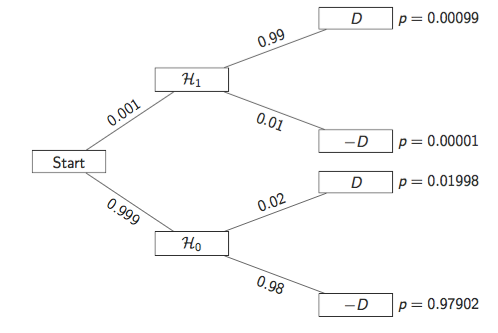
\includegraphics[width=.9\linewidth]{figures/week8/decisionTree.png}

Based on this tree, we can compute:

\begin{align*}
p(\mathcal{H_1}\mid D) & = \frac{p(D\mid \mathcal{H}_1)\cdot p(\mathcal{H}_1)}{p(D)}\\
&= \frac{0.99\cdot 0.001}{0.00099+0.01998}\\
&= 0.047
\end{align*}

Thus, even with VERY high accuracy, the very low prior probability of being a mutant makes it so that our posterior probability is only 4.7\% 

\section*{Building Bayesian models}
\label{sec-5}
Bayesian modeling uses the basic vocabulary of Bayes theorem.  Our goal is to quantify our \textbf{posterior beliefs} in a model.  We do this by \textbf{updating} our \textbf{prior beliefs} via Bayes theorem\ldots{}that is, posterior = prior x likelihood.

Let's revisit the "globe tossing" example from the first exam.

Suppose you have a globe that represents the Earth.  You would like to estimate how much of the surface is covered in water.  To measure this, you adopt the following strategy: toss the globe up in the air. When you catch it, you will record whether the surface under your right index finger is water or land.  Then you toss the globe up in the air again and repeat the procedure. The first nine samples generate the following sequence:

W L W W W L W L W

where W indicates water and L indicates land. So in this example you observe six W (water) observations and three L (land) observations. Call this sequence of observations the \textbf{data}.

To construct a model, we need to make assumptions.  Designing a simple Bayesian model uses a design loop with three steps.

\begin{enumerate}
\item Data story: Motivate the model by narrating how the data might arise.
\item Update: Educate your model by feeding it the data.
\item Evaluate: All statistical models require supervision, leading possibly to model revision.  We'll talk about this later.
\end{enumerate}

\subsection*{The data story}
\label{sec-5-1}
The "data story" amounts to explaining how each piece of data is born. This usually means describing aspects of the underlying reality as well as the sampling process. The data story in this case is simply a restatement of the sampling process:
\begin{itemize}
\item Assume the true proportion of water covering the globe is p.
\item A single toss of the globe has a probability p of producing a water (W) observation. It has a probability 1 − p of producing a land (L) observation.
\item Each toss of the globe is independent of the others.
\end{itemize}

This is usually translated into a probability statement, called a \textbf{likelihood}.  Based on the story, we can use a \textbf{binomial} likelihood to model the data generation.

\[
f(x,N,p) = \binom{N}{x}p^{x}(1-p)^{1-x}
\]

\subsection*{Updating}
\label{sec-5-2}

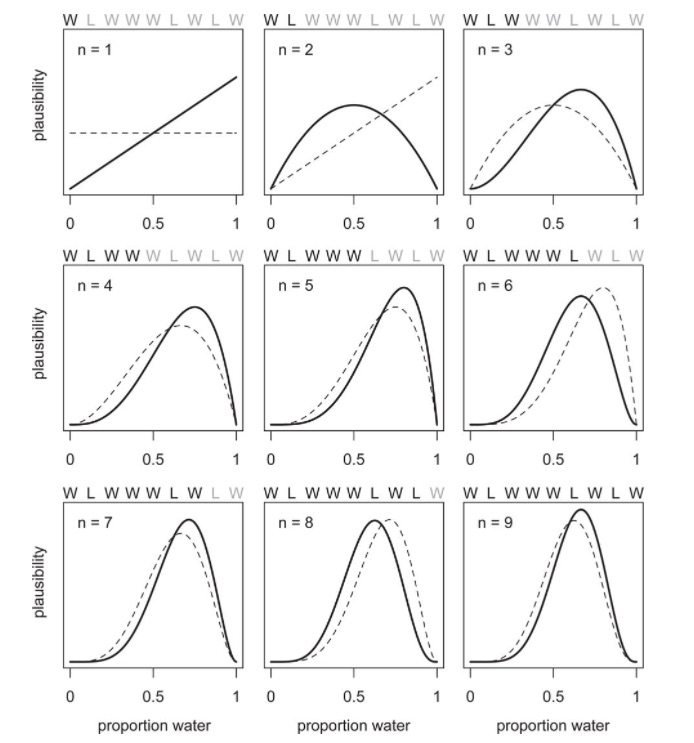
\includegraphics[width=.9\linewidth]{figures/week8/globeTossing.jpg}

In this figure, we see how Bayesian updating works.  
\begin{itemize}
\item start with a prior that assigns equal probability to all values of $p$ between 0 and 1.
\item after seeing the first "W", our posterior changes.  Now, $p=0$ is impossible (probability = 0), and $p>0.5$ is much more likely than $p<0.5$.
\item after seeing the next data "L", the posterior changes again.  Both $p=0$ and $p=1$ are impossible, with $p=0.5$ most likely (which makes sense, since out of TWO tosses, we've seen one W and one L).
\item after seeing the next data "W", the posterior again shifts toward $p=1$, but note that $p=1$ is still impossible.
\item each observation of "W" shifts the peak toward the right $p=1$, while each observation of "L" shifts the peak toward the left.
\end{itemize}

From this, we can think of a Bayesian model as a machine that:
\begin{itemize}
\item starts with a prior belief
\item takes in some data
\item updates the prior belief to a posterior belief.
\end{itemize}

Thus, all Bayesian models require a prior in order to function!  

\subsection*{Role of the prior?}
\label{sec-5-3}
This is where Bayesian modeling gets its most criticism.  In theory, you can use ANY prior you want.  Ideally, the prior you use should reflect your prior state of knowledge about the model.  

To see how the choice of prior can affect your posterior, consider the diagram below:

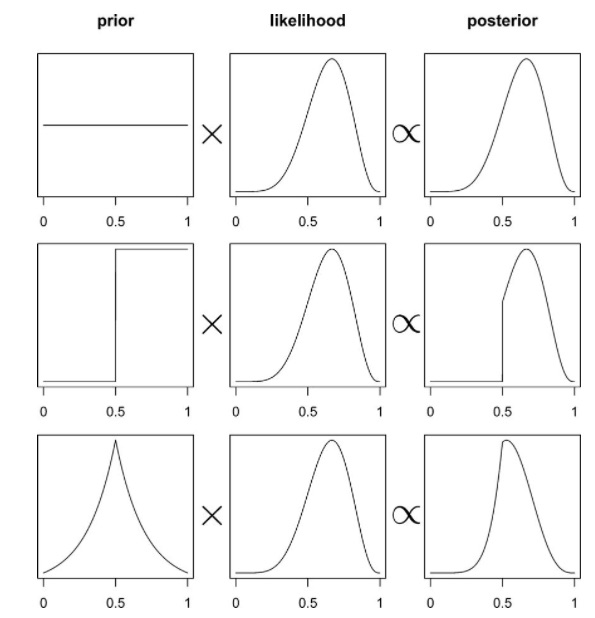
\includegraphics[width=.9\linewidth]{figures/week8/priors.jpg}

In the first row, we use a \emph{uniform prior}.  That is, each value of $p$ is equally likely.  When we multiply the prior by the likelihood, the resulting posterior looks the same as the likelihood.

In the second row, we use a different kind of prior.  Here, our prior belief is that $p$ MUST be larger than 0.5.  When multiplying by the likelihood, our resulting posterior belief still reflects this.  Notice that the posterior probability is still 0 for any $p<0.5$

Finally, in the third row, the peaked prior shifts and distorts the posterior (relative to the original likelihood).

\section*{Computations with Bayesian models}
\label{sec-6}
So far, we have concentrated on the conceptual side of Bayesian modeling.  That is, we've talked about what Bayesian models do (build posterior distributions based on priors and data).  We haven't actually talked about HOW to do these computations.  That's where we'll go next.

The mathematics behind Bayesian computation can get pretty complex.  Any course in mathematical statistics that does Bayesian computation will require knowledge of the integral calculus.

Fortunately, we now have modern computing methods that can do really good approximations for us.  As a first encounter, we'll talk about \textbf{grid approximation} today.

\subsection*{Grid approximation}
\label{sec-6-1}

Grid approximation works on the basis of dividing the "parameter space" (that is, all the values of $p$ we could consider) into a \emph{finite set} of points.  Then, we can define our prior and likelihood on this finite set of points, after which the posterior can be computed using simple arithmetic.  

Here's how it works:

\begin{enumerate}
\item Define the grid. This means you decide how many points to use in estimating the posterior, and then you make a list of the parameter values on the grid.
\item Compute the value of the prior at each parameter value on the grid.
\item Compute the likelihood at each parameter value.
\item Multiplying the prior by the likelihood.  This gives you the \emph{unstandardized} posterior at each parameter value on the grid
\item Finally, standardize the posterior (that is, turn it into a probability function).  This is done by dividing each value by the sum of all values.
\end{enumerate}

For our globe tossing example, the following code will accomplish each of these steps:

\begin{verbatim}
p_grid = seq(from=0, to=1, length.out=20)
prior = rep(1, 20)
likelihood = dbinom(x=6, size=9, prob=p_grid)
posterior = likelihood * prior
posterior = posterior/sum(posterior)
\end{verbatim}

We can plot the resulting posterior distribution as follows:

\begin{verbatim}
plot(p_grid, posterior, type="b")
\end{verbatim}

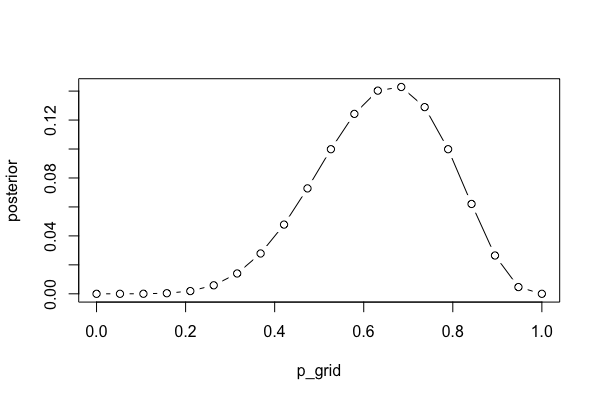
\includegraphics[width=.9\linewidth]{figures/week8/gridApproximation.png}

As an exercise, you should try using sparser grids (i.e., less than 20 points) and denser grids (i.e., more than 20 points).  What happens to your plot of the posterior?

Also, we can investigate the different priors we used earlier.  Re-run the code chunks above with the following definitions for \texttt{prior}:

\begin{verbatim}
prior = ifelse(p_grid < 0.5, 0, 1)
prior = exp(-5*abs(p_grid - 0.5))
\end{verbatim}

\subsection*{Using sampling to approximate posterior}
\label{sec-6-2}

In practice, most methods for computing posteriors rely on \textbf{sampling} from the posterior.  The idea is that once the model is built (i.e., once you've defined the prior and likelihood), we can estimate the posterior by pulling LOTs of samples, and then using those samples to answer questions that we care about.

To see how this works, we'll illustrate with our globe tossing model.

Let's start with a fairly dense grid approximation:

\begin{verbatim}
p_grid = seq(from=0, to=1, length.out=1000)
prior = rep(1, 1000)
likelihood = dbinom(x=6, size=9, prob=p_grid)
posterior = likelihood * prior
posterior = posterior/sum(posterior)
\end{verbatim}

The following code will pull 10,000 samples from the posterior distribution:

\begin{verbatim}
samples = sample(p_grid, prob=posterior, size=10000, replace=TRUE)
\end{verbatim}

We can see those samples here:

\begin{verbatim}
plot(samples)
\end{verbatim}

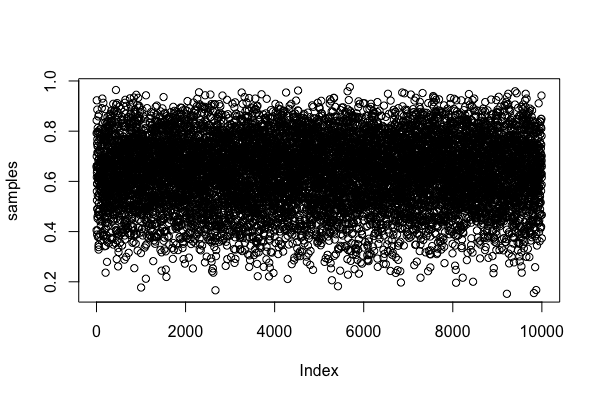
\includegraphics[width=.9\linewidth]{figures/week8/samples.png}

We can also plot the density of those samples.  Notice how closely it resembles our posterior plots from above.

\begin{verbatim}
plot(density(samples))
\end{verbatim}

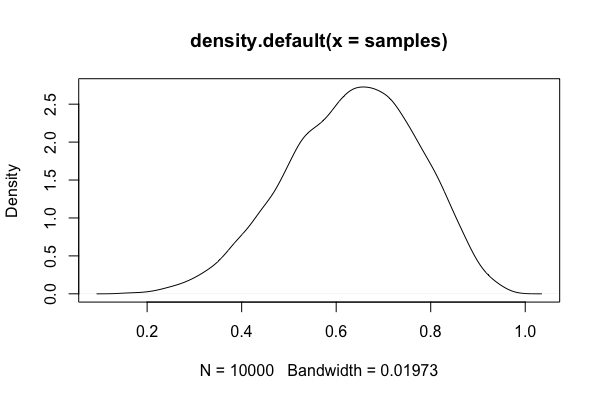
\includegraphics[width=.9\linewidth]{figures/week8/density.png}

\subsection*{Computations with posterior samples}
\label{sec-6-3}

Once we have our posterior samples, the model's work is done.  But your work as a modeler has just begun.  The next step is to \emph{summarize and interpret} the posterior distribution. Exactly how it is summarized depends upon your purpose. But common questions include:

\begin{itemize}
\item How much posterior probability lies below some parameter value?
\item How much posterior probability lies between two parameter values?
\item Which parameter value marks the lower 5\% of the posterior probability?
\item Which range of parameter values contains 90\% of the posterior probability?
\item Which parameter value has highest posterior probability?
\end{itemize}

These simple questions can be usefully divided into questions about (1) intervals of defined boundaries, (2) questions about intervals of defined probability mass, and (3) questions about point estimates. We'll see how to approach these questions using samples from the posterior.

\subsubsection*{Intervals of defined boundaries.}
\label{sec-6-3-1}

Suppose I ask you for the posterior probability that the proportion of water is less than 0.5. Using the grid-approximate posterior, you can just add up all of the samples where the corresponding parameter value is less than 0.5:

\begin{verbatim}
sum(samples<0.5)/10000
\end{verbatim}

We can also ask what proportion of the posterior distribution is between $p=0.5$ and $p=0.75$.

\begin{verbatim}
sum(samples>0.5 & samples<0.75)/10000
\end{verbatim}

\subsubsection*{Intervals of defined probability mass}
\label{sec-6-3-2}

Suppose instead I ask you for the 80th percentile of the posterior distribution:

\begin{verbatim}
quantile(samples,0.8)
\end{verbatim}

We can also do confidence intervals (usually called \emph{credible intervals} in Bayesian modeling).  For example, we can compute a 80\% confidence interval:

\begin{verbatim}
quantile(samples, c(0.1,0.9))
\end{verbatim}

In contrast to confidence intervals, the bounds of a 80\% \emph{credible interval} can be interpreted in terms of probability.  That is, there is a 80\% probability that $p$ is between 0.46 and 0.82.  This is not true for confidence intervals!

There is another type of interval estimate that we can compute with posterior samples: the \textbf{highest posterior density interval (HPDI)}.  The HPDI is defined as the narrowest interval containing the specified probability mass.  It is usually different from the 80\% credible interval, as we'll see in the following example.

Note: the code below will look a little more complicated.  That is because base R cannot do the HPDI computation.  However, the \texttt{coda} package can.  Since it works with MCMC samples (more on this later), we first have to convert our posterior samples to an MCMC sample.  Then, we can use the \texttt{HPDinterval} function:

\begin{verbatim}
library(coda)
sampMCMC = as.mcmc(samples)
HPDinterval(sampMCMC, prob=0.80)
\end{verbatim}

Compare the endpoints of the 80\% HPDI with the endpoints of the 80\% credible interval.

\subsubsection*{Point estimates}
\label{sec-6-3-3}
We can also just compute a mean or median:

\begin{verbatim}
mean(samples)
median(samples)
\end{verbatim}

However, if the posterior distribution is skewed, a mode might be better.  The drawback is that it is a little harder.  The idea of the code below is to compute the density of the samples, then find the $x$ value (i.e., the parameter value) that produces the highest density (\texttt{which.max}).

\begin{verbatim}
dens = density(samples)
dens$x[which.max(dens$y)]
\end{verbatim}

\section*{Summary}
\label{sec-7}
Today, we have described Bayesian modeling in terms of beginning with a model (a "data story") and using Bayes theorem to "update" the model with data.  Next time, we'll talk about how to \textbf{evaluate} our model by simulating data that should be implied by our model (the so-called \textbf{posterior predictive distribution}).  Finally, we will learn how to construct more complicated models, then proceed to use them for a lot of different applied problems.

For next time, you will need to install two pieces of software.  The first is JAGS, which can be found at \texttt{http://mcmc-jags.sourceforge.net/}.  Once you install this, you'll need to install the \texttt{R2jags} package in R by executing \texttt{install.packages("R2jags")}.
% Emacs 25.2.1 (Org mode 8.2.10)
\end{document}